% Autor: Leonhard Segger, Alexander Neuwirth
% Datum: 2017-10-30
\documentclass[
	% Papierformat
	a4paper,
	% Schriftgröße (beliebige Größen mit „fontsize=Xpt“)
	12pt,
	% Schreibt die Papiergröße korrekt ins Ausgabedokument
	pagesize,
	% Sprache für z.B. Babel
	ngerman
]{scrartcl}

% Achtung: Die Reihenfolge der Pakete kann (leider) wichtig sein!
% Insbesondere sollten (so wie hier) babel, fontenc und inputenc (in dieser
% Reihenfolge) als Erstes und hyperref und cleveref (Reihenfolge auch hier
% beachten) als Letztes geladen werden!

% Silbentrennung etc.; Sprache wird durch Option bei \documentclass festgelegt
\usepackage{babel}
% Verwendung der Zeichentabelle T1 (Sonderzeichen etc.)
\usepackage[T1]{fontenc}
% Legt die Zeichenkodierung der Eingabedatei fest, z.B. UTF-8
\usepackage[utf8]{inputenc}
% Schriftart
\usepackage{lmodern}
% Zusätzliche Sonderzeichen
\usepackage{textcomp}

% Mathepaket (intlimits: Grenzen über/unter Integralzeichen)
\usepackage[intlimits]{amsmath}
% Ermöglicht die Nutzung von \SI{Zahl}{Einheit} u.a.
\usepackage{siunitx}
% Zum flexiblen Einbinden von Grafiken (\includegraphics)
\usepackage{graphicx}
% Abbildungen im Fließtext
\usepackage{wrapfig}
% Abbildungen nebeneinander (subfigure, subtable)
\usepackage{subcaption}
% Funktionen für Anführungszeichen
\usepackage{csquotes}
% Zitieren, Bibliographie
\usepackage{biblatex}


% Zur Darstellung von Webadressen
\usepackage{url}
%chemische Formeln
\usepackage[version=4]{mhchem}
% siunitx: Deutsche Ausgabe, Messfehler getrennt mit ± ausgeben
\usepackage{floatrow}
\floatsetup[table]{capposition=top}
\usepackage{float}
% Verlinkt Textstellen im PDF-Dokument
\usepackage[unicode]{hyperref}
% "Schlaue" Referenzen (nach hyperref laden!)
\usepackage{cleveref}
\sisetup{
	locale=DE,
	separate-uncertainty
}
%\bibliography{6Mi_M3_29-11-2017_References}
%TODO anpassen

\begin{document}
	
	\begin{titlepage}
		\centering
		{\scshape\LARGE Versuchsbericht zu \par}
		\vspace{1cm}
		{\scshape\huge A3 - Absorption von Beta- und Gamma-Strahlung \par}
		\vspace{2.5cm}
		{\LARGE Gruppe 14Mo \par}
		\vspace{0.5cm}
		
		{\large Alexander Neuwirth (E-Mail: a\_neuw01@wwu.de) \par}
		{\large Leonhard Segger (E-Mail: l\_segg03@uni-muenster.de) \par}
		\vfill
		
		durchgeführt am 07.05.2018\par
		betreut von\par
		{\large Johann Preuß}  
		
		\vfill
		
		{\large \today\par}
	\end{titlepage}
	\tableofcontents
	\newpage

	\section{Kurzfassung}
	%TODO Hypothese	und deren Ergebnis, wenn Hypothese ist, dass nur Theorie erfüllt, sagen: Erwartung: Theorie aus einführung (mit reflink) erfüllt
	%TODO Ergebnisse, auch Zahlen, mindestens wenn's halbwegs Sinn ergibt
	%TODO Was wurde gemacht
	%TODO manche leute wollen Passiv oder "man", manche nicht
	In diesem Versuch wurde die Absorption von Beta- und Gammastrahlung untersucht. %überflüssig?
	Dazu wurde der Zusammenhang zwischen Schichtdicke eines Absorbers, Art der Strahlung des Präparats und Impulsrate betrachtet.
	
	\section{Methoden}\label{Methoden}
	%TODO Bilder von der Website klauen
	Der Versuchsaufbau bestand aus einem Geiger-Müller-Zählrohr, das an ein Betriebsgerät angeschlossen war.
	Vor das Glimmerfenster des Zählrohrs konnten nun verschiedene radioaktive Präparate installiert werden und unterschiedliche Absorber zwischen Präparat und Röhre gebracht werden.
	
	Zunächst wurde die Zählrohrcharakteristik des Geiger-Müller-Zählrohres bestimmt, um die folgenden Untersuchungen im Plateaubereich der Zählrohrkennlinie durchführen zu können.
	Dazu wurde die Impulsrate des Zählrohrs mit $\beta$-Präparat bei steigender Zählrohrspannung bestimmt.
	Begonnen wurde hier unmittelbar unter der Einsatzspannung und die folgenden Messungen wurden bei ca. \SI{100}{\volt} über der Einsatzspannung durchgeführt.
	
	Dann wurde, um die mittlere Untergrundaktivität zu bestimmen, 200 mal die Zahl der Untergrundimpulse in \SI{10}{\second} gemessen.
	Anschließend wurde die Impulsrate des $\gamma$-Präparats mit zunehmender Schichtdicke des Blei-Absorbers gemessen und die Impulsrate des $\beta$-Präparats mit zunehmender Aluminium-Absorber-Dicke.
	Zuletzt wurde noch die Impulsrate des $\beta$-Präparats mit Plexiglas- und Gummiabsorber bei konstanter Schichtdicke bestimmt.
	
	Hierbei wurden jeweils mindestens 1111 Impulse gemessen, um die relative Unsicherheit unter 3\% zu halten.
	Die Betriebsspannung wurde vom Betriebsgerät abgelesen und nicht mit einem externen Voltmeter überprüft.
	
	%TODO Bestimmen der Zählzeit => 1111 Impulse
	
	\section{Ergebnisse und Diskussion}
	%TODO Datenanalyse -> Überschrift?
	%TODO Unsicherheiten
	

	\subsection{Beobachtung}
	%TODO Einflüsse von veränderten Parametern auf Messung
	In \cref{Zaehlrohrcharakteristik} ist die Impulsrate gegen die Zählrohrspannung aufgetragen.
	bei ca. \SI{313}{\volt} steigt die Impulsrate abrupt von 0 auf 9 Impulse pro Sekunde und ändert sich danach nur noch unwesentlich. %Zahlen ausschreiben?

	
	%TODO mehr!
	
	\begin{figure}[H]
		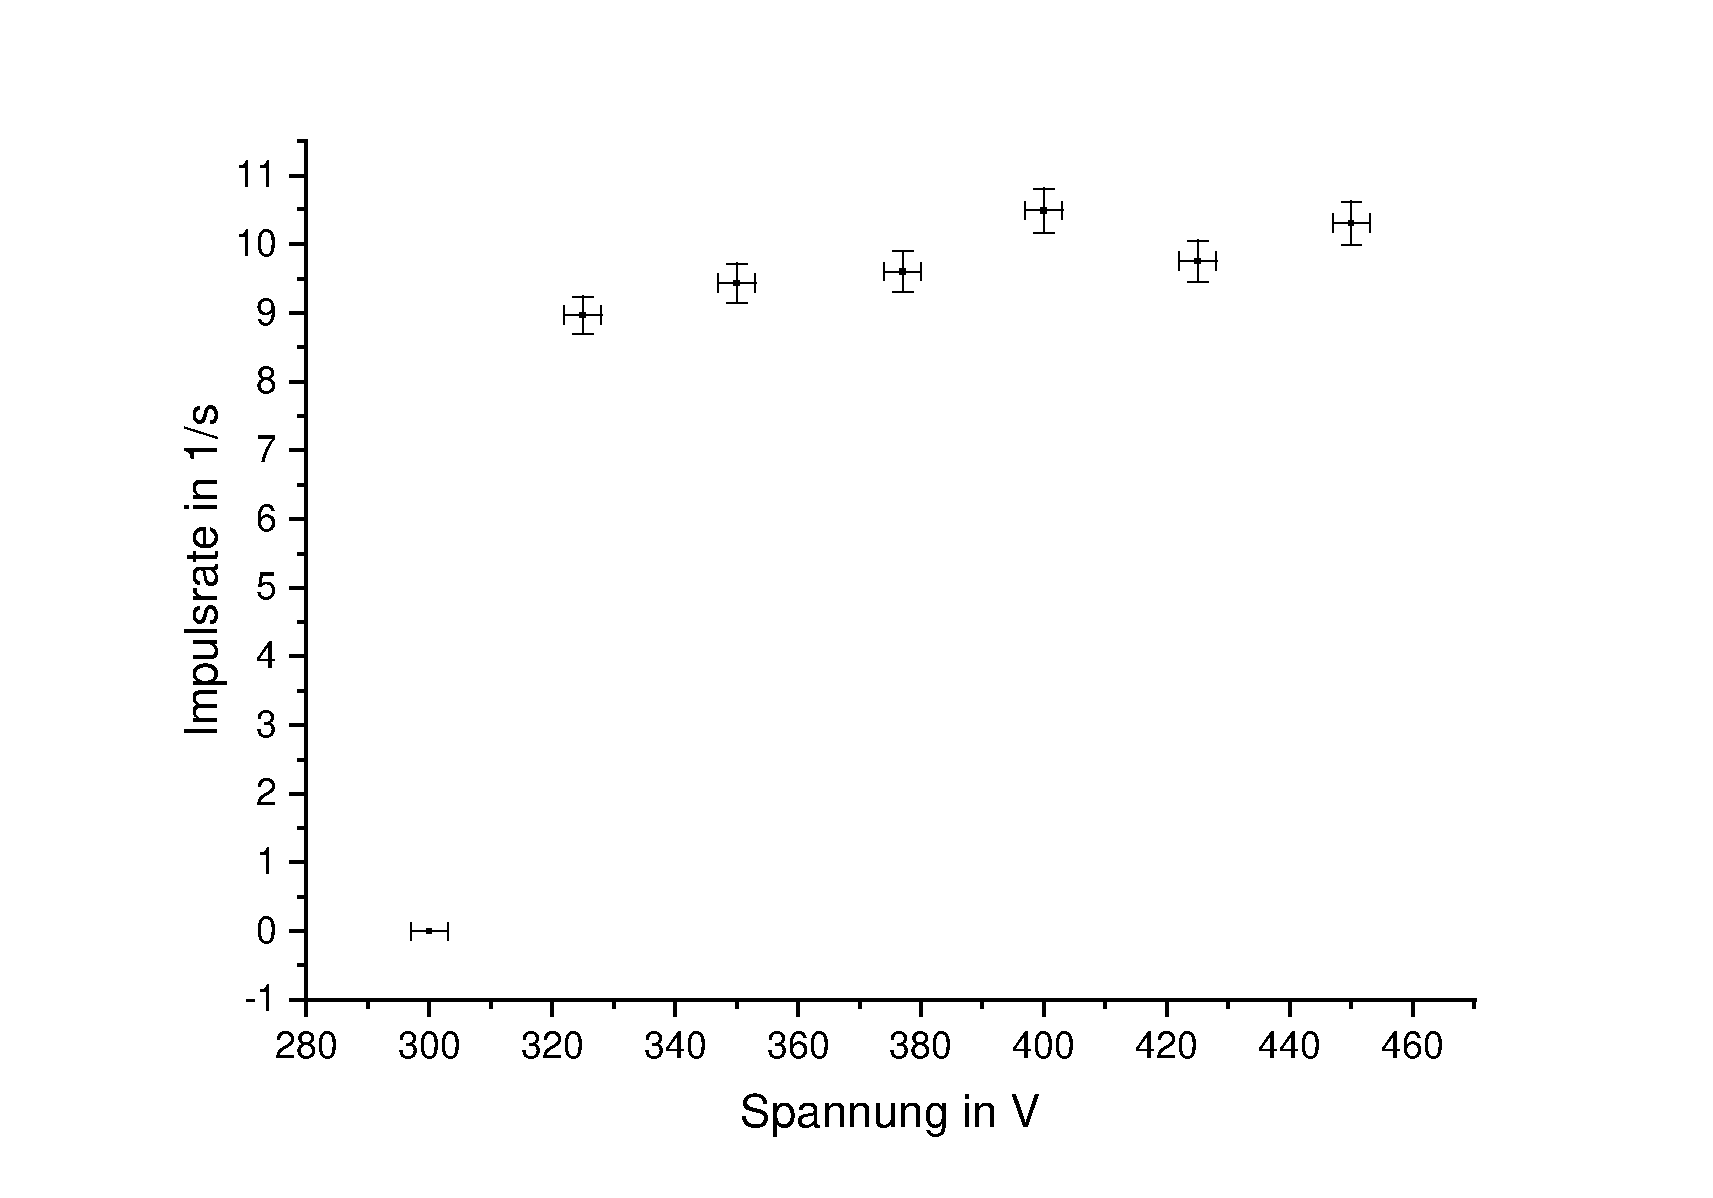
\includegraphics[width=0.7\textwidth]{Zaehlrohrcharakteristik}
		\centering
		\caption{Aufgenommene Zählrohrcharakteristik. Mit $\beta$-Präparat.}%TODO Titel
		\label{Zaehlrohrcharakteristik}
		\centering
	\end{figure}

	\subsubsection{Unsicherheiten} %TODO Schon alles?
	Die Unsicherheit der Betriebsspannung des Geiger-Müller-Zahlrohrs beträgt \SI{3}{V} (Dreieckverteilung).  
	Die Zählzeit wurde in Sekunden auf einer Digitalanzeige gestoppt wodurch sich eine Unsicherheit von \SI{0,6}{s} ergibt (Rechteckverteilung).
	Wie in \cref{Methoden} beschrieben ist die relative Unsicherheit der Impulsmessungen kleiner 3\%.
	\subsection{Datenanalyse}
	\subsubsection{Untergrundpulse}
	Die Messung der Untergrundimpulse über 200 mal 10 Sekunden ergab einen Mittelwert von 2,685 Impulsen und eine Standardabweichung von 1,519. 
	In \cref{Untergrund} sind die absolute und relative Häufigkeitsverteilungen dargestellt, da sich die Ordinatenwerte lediglich um einen Faktor von 200 unterscheiden lässt sich an der linken Achse die absolute und an der rechten die relative Häufigkeit ablesen.
	Des Weiteren ist in \cref{Untergrund} die Poisson-Verteilung für $\bar{N}$ = 2,685 abgebildet.
	\begin{equation}
		\psi(N) = \frac{\bar{N}^N \cdot e^(-\bar{N})}{N!}
	\label{Poisson}
	\end{equation}
	
	\begin{figure}[H]
		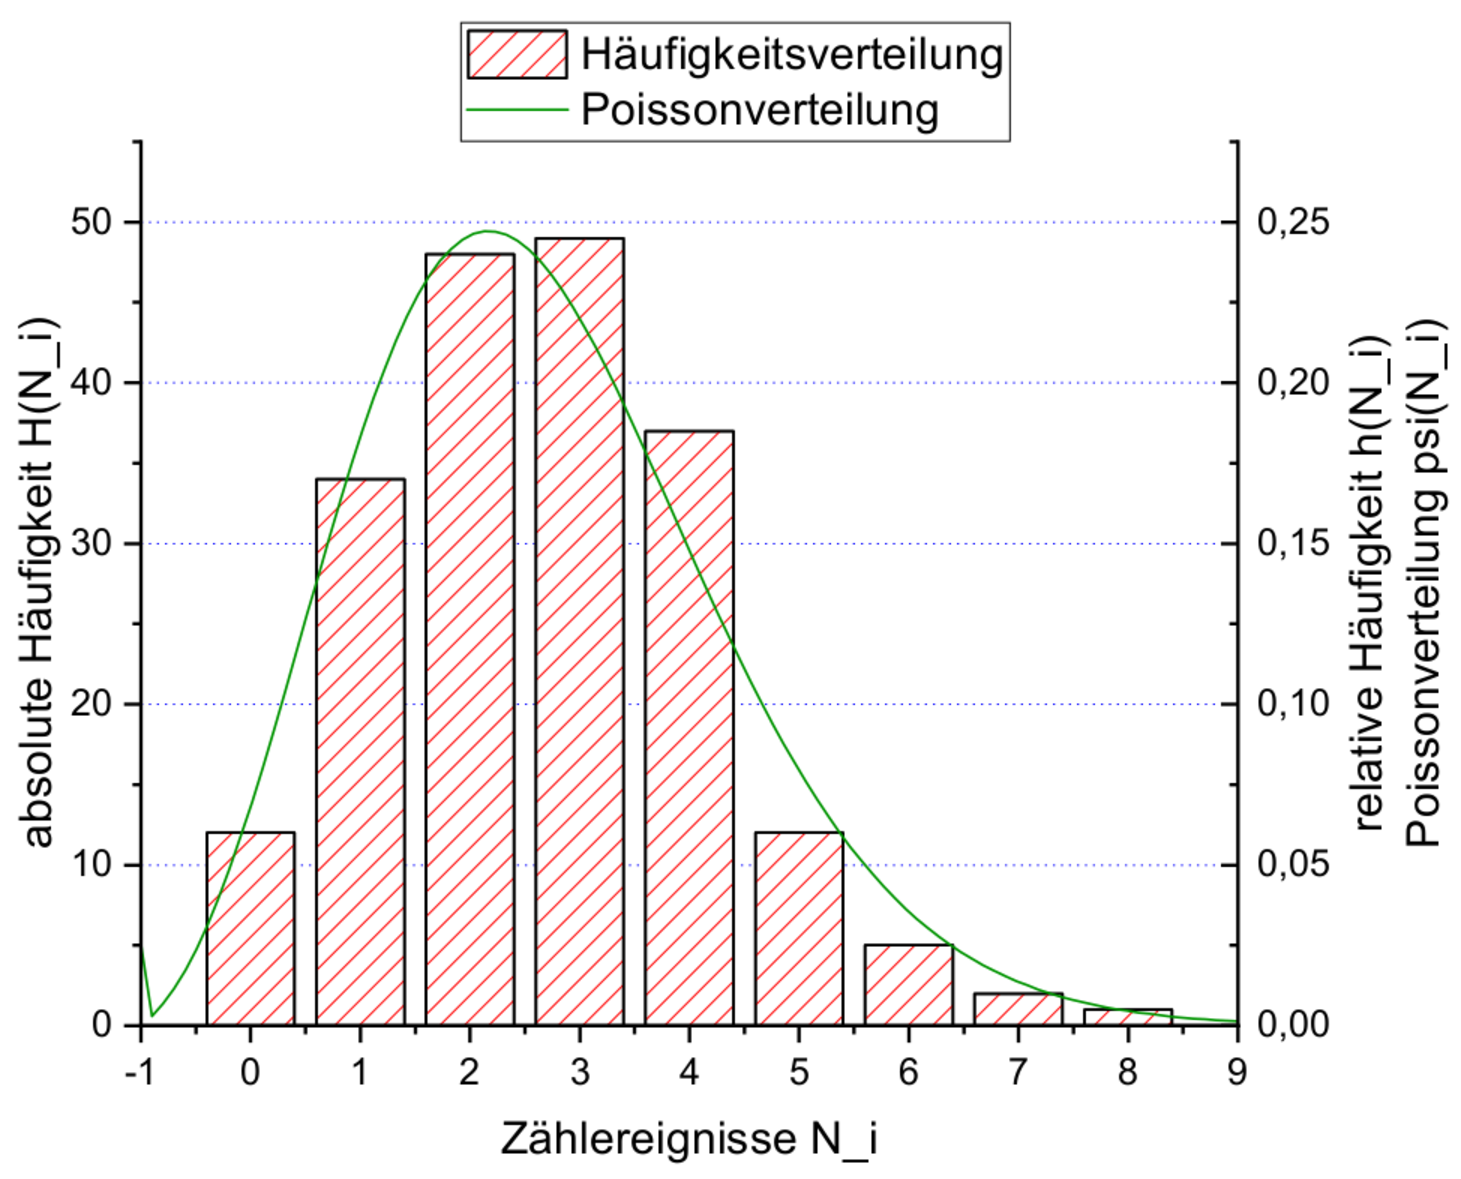
\includegraphics[width=0.7\textwidth]{Untergrund}
		\centering
		\caption{Aufgenommene absolute und relative Häufigkeitsverteilung der Untergrundpulse. Außerdem ist die durch deren Mittelwert festgelegte Poisson-Verteilung abgebildet.}%TODO Titel
		\label{Untergrund}
		\centering
	\end{figure}
	\subsection{Diskussion}
	%TODO Bezug/Nutzten oder sonst was
	%TODO auch hier die Hypothese wiederholen
	%TODO keine Messwerte hier, nach manchen Menschen, zumindest "direkt" erstellte Diagramme net hier, auch wenn Lesbarkeit-bla
	Es ist ersichtlich, dass die Einsatzspannung des Zählrohrs zwischen 300 und \SI{325}{V} liegt. %lieber 2x SI?
	Auch das für Zählrohrkennlinien typische Plateau ist in \cref{Zaehlrohrcharakteristik} deutlich erkennbar.
	Der starke Anstieg vor dem Plateau konnte nicht aufgelöst werden und das Betriebsgerät verhinderte eine Erhöhung der Spannung auf Werte, die eine selbstständige Gasentladung zur Folge hätten.
	
	Da im $\beta$-Präparat zwei Zerfälle stattfinden, die beide $\beta$-Strahlung produzieren, war eine Überlagerung aus aus Absorptionskurven von Elektronen aus dem Strontium- und aus dem Yttriumzerfall zu erwarten.
	Aus dem linearen Zusammenhang in der logarithmischen Darstellung lässt sich erkennen, dass nur einer der Zerfälle einen messbaren Einfluss auf die Zerfallskurve hat, da sich ansonsten eine Überlagerung zwei Geraden unterschiedlicher Steigung ergeben hätte.
	Dies liegt vermutlich daran, dass sich das Präparat selbst nicht an der Oberfläche des Präparathalters, sondern hinter eine Abdeckung befand, die die niederenergetischen Elektronen des Strontiumzerfalls nicht durchdringen konnten.
	
	\section{Schlussfolgerung}
	%TODO Rückgriff auf Hypothese und drittes Nennen dieser
	
	%TODO Quellen zitieren, Websiten mit Zugriffsdatum
	%TODO Verweise auf das Laborbuch (sind erlaubt)
	%TODO Tabelle + Bilder mit Beschriftung
	%\printbibliography
\end{document}
